% Este archivo es parte de la memoria del proyecto fin de carrera
% de Aarón Bueno Villares. Protegida bajo la licencia GFDL.
%
% Para más información, la licencia completa viene incluida en el
% fichero fdl-1.3.tex

% Copyright (C) 2010 Aarón Bueno Villares

\section{Análisis y diseño del sistema}
\label{sec:diseno}

\subsection{Confección del reglamento}
Se pueden forjar muchas preguntas sobre qué va a tener un juego de
táctica militar. A su vez, se pueden forjar otras tantas acerca de qué
va a tener un juego de corte fantástico. En suma, hay una gran
diversidad de preguntas por contestar.

Aquí se muestra un grupo de ellas:
\begin{itemize}
\item \emph{¿Qué razas estarán disponibles?}
\item \emph{¿Qué elementos de una batalla real vamos a considerar?}
\item \emph{¿Sobre qué tipo de terrenos se va a combatir?}
\item \emph{¿Cómo se organizará cada ejército?}
\item \emph{¿Con cuántos elementos fantásticos se trabajará?}
\item \emph{¿Qué tiempo de batalla real representará cada turno de
    juego?}
\item \emph{¿Cómo representaremos la escena y con qué elementos de
    escenografía contaremos?}
\item \emph{¿Cómo modelaremos las capacidades de cada ``soldado''?}
\end{itemize}

Todas estas preguntas han necesitado responderse a fin de confeccionar
un reglamento consistente. Por otro lado, si bien es cierto que
\gomf, por el simple hecho de ser un juego basado en turnos, no
constituye una simulación real de ninguna batalla campal, sí que es una
buena aproximación esquemática de su contenido (podría aplicarse aquí el
calificativo de simulación conceptual).

Este factor hace falta tenerse en cuenta para crear un reglamento
coherente. Intentar modelar aspectos que son demasiado característicos
del \emph{tiempo real} en una serie de turnos puede resultar
artificial. Así, no deberíamos sentirnos incómodos si decidimos
ordenar en un mismo turno acciones que ocurren
simultáneamente. Es el precio a pagar si queremos diseñar un juego
basado en turnos.

Por último, en una batalla ocurre una gran multitud de cosas. No
podemos, \emph{a priori}, considerarlas todas. Por ello, también
veremos adecuado forjarnos ciertas fronteras funcionales; por
cuestiones de viabilidad.

La muestra final de este reglamento se encuentra en el anexo
\ref{reglamento}.

\subsection{Arquitectura general del sistema}
Como hemos venido mencionando, nuestro juego está basado en un
reglamento. Existirá, por tanto, una entidad encargada de gestionar
dicho reglamento. Ésta será la parte lógica de nuestro sistema. Por
otro, es necesario una interacción con el usuario donde poder elegir
las acciones que, en cada momento de la partida, ofrece \gomf.

A fin de organizar el diseño en la clásica arquitectura de capa de
presentación y capa de dominio, hemos considerado, primeramente, dos
clases principales: \emph{gestor de interfaz} y \emph{gestor de
  reglas}.

Está claro que la capa de dominio es representada completamente por
el reglamento, comprendiendo la capa de presentación su interfaz de
interacción con el usuario. El
\emph{gestor de reglas} es el resposanble pues, de la capa de dominio,
y el \emph{gestor de interfaz} de la capa de presentación.

El \emph{gestor de interfaz}, a parte de disponer al usuario del menú
principal del juego y la confección de ejércitos, se encarga, una vez
dentro de una batalla, de mostrar al usuario todas las acciones
disponibles, responder a las peticiones del usuario y mostrar los
cambios producidos por éstas. También gestiona el sonido del juego.

Y por último, para hacer efectiva esa interacción entre ambas clases,
dispondremos de otras dos, la clase \emph{estado}, que encapsulará la
información usada como \emph{testigos} pasados en los cambios
producidos dentro de cada capa, y la clase \emph{juego}, la de más
alta jerarquía en el juego, que se encargará de encapsular a los
gestores.

\begin{figure}[h]
\centering
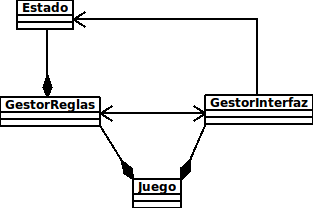
\includegraphics[scale=.8]{./imagenes/DiagramaJuego.png}
\label{fig:arqgen}
\caption{Arquitectura general del sistema (UML)}
\end{figure}

El proceso global y principal del juego es el siguiente:

\begin{enumerate}
\item Al lanzar el juego, la clase \emph{juego} inicializa al gestor
  de interfaz y lanza su menú.
\item Los deseos del usuario (la opción elegida del menú) se devuelven
  a la clase \emph{juego} para que actúe en consecuencia.
\item Si se eligió comenzar una batalla, los usuarios eligen los
  dos ejércitos combatientes y la clase \emph{juego}, acto seguido,
  inicializa al \emph{gestor de reglas} (acto que da comienzo a la
  partida).
\item El \emph{gestor de reglas} entrega al \emph{gestor de interfaz}
  el estado inicial del juego.
\item Con esa información el gestor de interfaz imprime
la situación actual de la batalla y ofrece al usuario todas las
acciones disponibles para continuar jugando, información que se
obtiene también del \emph{estado}.
\item Si el usuario realiza alguna acción, la interfaz envía esa
  información al \emph{gestor de reglas}.
\item El gestor de reglas modifica con esa información
  el estado interno del juego.
\item Se repite el proceso hasta que el gestor de interfaz
  reciba un estado final.
\item Tras esto, se muestra el resultado de la partida y se vuelve al
  menú principal del juego.
\end{enumerate}

\subsection{Capa de dominio}
\subsubsection{Estado y acciones}
El reglamento indica que existen seis turnos para cada jugador, y
cada turno se divide en dos fases: movimiento y combate. Por último,
cada fase se divide en ciertas subfases, donde se pueden realizar
ciertas acciones.

Consideraremos que una \emph{acción} posee un nombre o etiqueta, que
llamaremos \emph{tarea}, mas toda la información necesaria para que esa
acción pueda ejecutarse. Por ello, tendremos una enumeración que
contendrá la lista de etiquetas de las acciones disponibles, y una
clase concreta para cada acción, cuyos atributos serán los datos
necesarios para que dicha acción pueda realizarse. Por ejemplo, para
la acción \emph{declaración de carga}, su único atributo será la
unidad objetivo (luego el gestor de reglas evaluará si esa carga será
efectiva o fállida, pero con esa información la acción queda
completamente definida).

Evidentemente, existe cierto comportamiento e información genérica que
comparten todas las acciones concretas, como la fase sobre la que está
definida, o la tarea que la etiqueta. Por ello, existirá una clase
base llamada acción, y una clase heredada por cada acción posible en
\gomf. A su vez, cada clase heredada (cada acción concreta) añadirá el
conjunto de atributos adicionales necesarios para su propia
definición.

\begin{figure}[h]
\centering
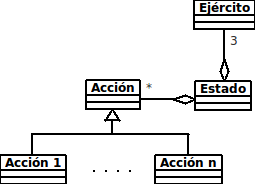
\includegraphics[scale=.8]{./imagenes/Estado.png}
\label{fig:estado}
\caption{Clase estado y clase acción (UML)}
\end{figure}

Con respecto al estado, contendrá toda la información necesaria y
relativa a un estado concreto de la partida: jugador actual, turno
actual, así como la fase y subfase actual del turno del jugador en
curso.

Pero esto solo define a un estado, quizás, desde el punto de vista del
reglamento. Desde el punto de vista de nuestra jerarquía de clases, un
estado concreto de juego es definido por mas aspectos.

La interfaz tiene como su única fuente de información el tipo estado,
y como se ha de imprimir la situación actual de los ejércitos
involucrados (los dos ejércitos combatientes, y el ejército GAIA), el
tipo estado también debe proveerlo.

Por último, aunque la interfaz conozca todas las acciones existentes,
no necesariamente debe conocer cuando sí y cuando no están
disponibles cada una de ellas. El \emph{gestor de reglas} es la
entidad encargada de mantener actualizada esta información en el
estado a medida que transcurre la partida, para que luego la interfaz
tenga acceso a él y disponga al usuario la disponibilidad funcional
actual correcta.
%%TODO: Gráfico de estado con ejército y lista de acciones tareas.

\subsubsection{Ejército y unidades}
El tipo unidad es el tipo básico sobre el cual gira \gomf. Existen
solamente dos razas distintas, y cada raza tiene en concreto nueve
unidades distintas\footnote{El hecho de que sean nueve no es por
  ninguna razón concreta, sencillamente es el límite que la
  imaginación me impone.}.

Toda modificación de la posición de una unidad, su número de
efectivos, y toda información referida a ella está poseida en la
propia clase, como era de esperar. A su vez, la clase ejército es,
básicamente, la encapsulación de una serie de unidades que pertenecen
al mismo bando, y fundamentalmente no contiene ninguna información
adicional.

Existirá, por tanto, un tipo heredado particular para cada una de las
razas, y un tipo heredado particular para cada uno de las unidades de
cada raza.

\begin{figure}[h]
\centering
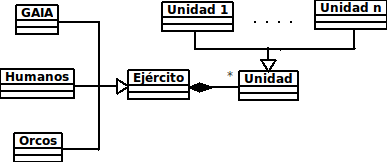
\includegraphics[scale=.8]{./imagenes/Ejercitos.png}
\label{fig:ejercitos}
\caption{Clase ejército y clase unidad (UML)}
\end{figure}

\paragraph{GAIA}
Usualmente, en muchos juegos de estrategía, se cuenta con un ejército
especial llamado ``GAIA'' que es transparente al jugador, y es usado
por la aplicación para gestionar el comportamiento general del
escenario de juego.

Esto se hace evidente en algunos juegos que tienen un editor de
escenarios. Por ejemplo, en el juego \emph{Tzar}, un juego de
estrategía de la compañia \emph{FX}, se disponía de distintos menús,
uno para cada equipo de la partida que estuvieses diseñando, que te
permitía colocar en el mapa los elementos disponibles del mismo:
edificios, unidades, objetos, etc. Y, a su vez, disponía de un
``equipo'' adicional llamado GAIA, y con él, se podían añadir
montañas, bosques, animales, minas de recursos, etc.

En \gom hemos adoptado la misma convención, y para los elementos de
escenografía hemos utilizado la estructura general de la clase
\emph{ejército} para crear un nuevo ejército llamado \emph{GAIA}.

La ventaja de usar GAIA como ejército es que los elementos de
escenografía son tomadas entonces como unidades, lo que nos permite hacer
un trato directo de estos elementos para realizar los cálculos sobre
visibilidad de las unidades o las capacidades de movimiento de las
mismas, ya que dichos elementos escenográficos son tratados como
elementos impasables y además, ocultan la visibilidad del mismo modo que
cualquier otra unidad.

\subsubsection{Gestor de reglas}
El gestor de reglas, mas que una clase, es una entidad compuesta por
una serie de clases que gestionan las acciones ejecutadas y
que mantiene el control del reglamento.

Estrictamente hablando, el gestor de reglas es una única clase muy
general que solo ejecuta una serie de acciones básicas. El núcleo de
la funcionalidad recae sobre otras clases concretas específicas para
cada fase.

\begin{figure}[h]
\centering
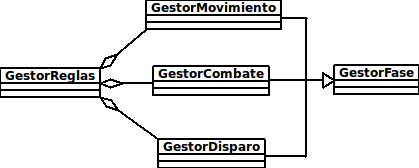
\includegraphics[scale=.8]{./imagenes/Reglas.png}
\label{fig:reglas}
\caption{Gestor de reglas (UML)}
\end{figure}

Sin embargo, podemos usar indistintamente el término entidad o clase
\emph{gestor de reglas} para referirnos a la entidad concreta ya que
dicha clase funciona como un API de toda la entidad. De este modo,
toda acción recibida se envía al gestor de reglas, y si hace falta
transmitir dicha información a una clase de fase específica, el gestor
de reglas se encargara de ello, y nunca la interfaz, ni ninguna clase
intermediaria o auxiliar tendrá acceso a ellas.

El proceso es el siguiente:
\begin{enumerate}
\item El gestor de reglas recibe una nueva acción.
\item Si la acción es una acción general\footnote{Las acciones se
    jerarquizan en tres clases: acciones de movimiento, acciones de
    combate, y acciones generales. Las acciones generales son todas
    aquellas que no se pueden emarcar en ninguna de las dos
    anteriores, por ejemplo, la elección de una unidad o el comienzo
    de un nuevo turno.}, es gestionada directamente por el gestor.
\item Si no es una acción general, y es una acción de la misma fase
  que la actual, se pasa el control a dicha clase de fase, junto al
  estado actual y el gestor de escenario -de este modo, la fase
  correspondiente tiene todas las herramientas necesarias para
  evaluar y ejecutar la acción-.
\item Si no es una acción general, pero la fase a la que pertenece la
  acción no coincide con la fase en curso, no se produce ningún cambio
  en el estado de juego.
\end{enumerate}

En concreto, existirán tres gestores de fases, el \emph{gestor de
  movimiento}, el \emph{gestor de combate} y el \emph{gestor de
  disparo}, cada una encargada de gestionar el desarrollo de cada
fase. Como pasaba con el tipo acción, existe cierto comportamiento
genérico común de dichas clases de fase, así como por el trato dado
por el gestor de reglas. En definitiva, dichas clases serán herencias
concretas de una clase base llamada \emph{gestor de
  fase}\footnote{Este \emph{convenio} permite, además, 
  aumentar la escalabilidad del producto, ya que se automatiza en
  parte la inclusión de nuevas fases futuras, como puede ser el
  disparo o la magia.} \footnote{La relación incluida en el gráfico,
  entre el gestor de movimiento y el de combate, existe debido a que
  es necesaria cierta comunicación entre ambos gestores cuando se
  realizan nuevas cargas, que implican nuevos combates -o cambios
  sobre los combates existentes en la fase de movimiento-.}

\subsubsection{Gestor de escenario y matemáticas}
Esta clase es una clase excepcional que no es intermediaria entre la
entidad de reglas y de interfaz, pero que son requeridas por igual por
ambas, y en concreto, por la clase \emph{GestorMovimiento} y
\emph{GestorInterfaz}.

Es aquella que provee toda la funcionalidad necesaria para
realizar acciones que dependen de la situacion de una unidad respecto
al resto de unidades, es decir, la única que trabaja considerando al
conjunto de unidades y el espacio -escenario- donde éstas residen.

Por ejemplo, en esta clase se calcula si una unidad ve
\refreg{visibilidad} a otra unidad, ya que dicha visibilidad depende
del resto de unidades presentes en el escenario. Si existen unidades
en el camino de una unidad a otra, o la unidad objetivo está en alguna
posición fuera del rango de visibilidad de la primera, la función 
miembro correspondiente de la clase devolverá si es cierto o no que
dicha visibilidad exista. Ocurre lo propio en el movimiento de carga,
el movimiento de huida, o la distancia máxima de movimiento o
pivotaje.

Por último, existe un \emph{módulo}\footnote{Lo notamos como módulo
  porque no es una clase única con una serie de funciones miembro,
  sino una serie de estructura y funciones independientes -aunque
  interrelacionadas-.}, llamado matemáticas, que provee una serie de
estructuras y funciones, principalmente geométricas -idoneas sobre
todo para la naturaleza de los cálculos realizados por el gestor de
escenarios-, que son las únicas que necesitamos para estos
cálculos.

\begin{figure}[h]
\centering
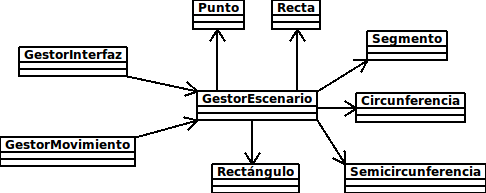
\includegraphics[scale=.8]{./imagenes/Escenario.png}
\label{fig:escenario}
\caption{Gestor de escenario y módulo matemático (UML)}
\end{figure}

\subsection{Capa de presentación}
\subsubsection{Gestor de interfaz}
Al igual que pasaba con el gestor de reglas, esta clase funciona como
API para toda la entidad de interfaz, compuesta por una serie más
compleja de clases.

El comportamiento del gestor de interfaz se puede dividir en tres
\emph{partes} fundamentales:
\begin{itemize}
\item Control de menú.
\item Gestión de ejércitos.
\item Interfaz de batalla.
\end{itemize}

El control del menú es controlado directamente por el gestor de
interfaz. La gestión de los ejércitos (creación y edición de
ejércitos), está completamente controlada por la clase \emph{gestor de
  ejércitos}. Y por último, la interfaz de batalla es controlada por
el propio gestor de interfaz pero esta vez ayudada por el \emph{gestor
  de iconos} para la gestión, muestra y captura de iconos y captura
(que no procesamiento) de acciones elegidas por el usuario (y como ya
hemos mencionado, por el \emph{gestor de escenario} para realizar los
cálculos involucrados).

\begin{figure}[h]
\centering
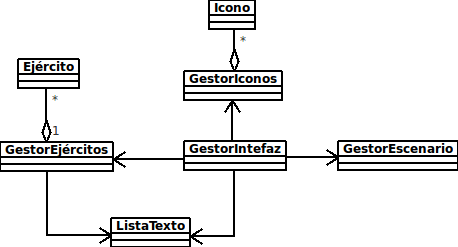
\includegraphics[scale=.8]{./imagenes/Interfaz.png}
\label{fig:interfaz}
\caption{Gestor de intefaz (UML)}
\end{figure}

\subsubsection{Lista de textos}
Es una clase auxiliar usada por el control de menú y la gestión de
ejércitos que provee una especie de \emph{motor} para trabajar con
listas de elementos textuales que te permiten seleccionar, etiquetar,
añadir y eliminar los distintos ítems que pueden formar las listas.

Por ejemplo, si el usuario hace click en un item de la lista, se
imprime una imagen sobre dicho item para
indicar que ha sido seleccionado (dicha imagen será pasada por el
usuario en la contrucción de la lista). Si la lista contiene mas items
que los permitidos para visualizar a la vez, se imprime un scroll para
poder desplazarte por la lista, o si se indica que se desea etiquetar
un item, se desplaza el item para dejar hueco a la etiqueta, de modo
que el conjunto quede nuevamente centrado.

Esta clase resulta muy útil para gestionar, sobre todo, el menú
contextual de la edición y creación de ejércitos, usado para imprimir
la lista de unidades disponibles de una raza dada, la lista de razas
disponibles, el sumario de la configuración actual del ejército, o la
lista de ejércitos creados.

\subsubsection{Gestor de ejércitos}
Es la clase encargada de controlar y mantener, mediante menús para el
usuario, el conjunto de ejércitos existentes, eliminarlos o crear
ejércitos nuevos, así como 
modificarlos y elegirlos cuando comienza una batalla. Comprueba,
además, que los ejércitos creados o modificados sean correctos (que no
existan unidades fuera de la zona de despliegue o \emph{pisándose} en
dicha zona de despliegue), o que los ejércitos elegidos de un combate
estén equilibrados en puntos, tal y como indica el reglamento de
\gomf.

Debido a la simplicidad de un ejército, la información de los
ejércitos existentes es guardada en ficheros de texto plano
simples. En ellos se guarda la lista completa de ejércitos, y el
contenido de cada uno de ellos.

\subsubsection{Gestor de iconos}
Un icono es un elemento contextual que identifica a una acción
concreta. Así, el gestor de iconos imprime la secuencia de iconos
correspondientes a las acciones disponibles\footnote{En realidad,
  imprime las acciones activas mas las disponibles.}, además de
proveer una descripción de cada icono, como ayuda contextual para el
usuario.

La forma de actuar del gestor de iconos es la siguiente:
\begin{enumerate}
\item Se obtiene, a partir del estado, la lista de acciones
  activas.
\item Se imprimen todos los iconos, distinguiéndose los que están
  disponibles de los que no, en zonas separadas de la zona de iconos.
\item Si el ratón se situa sobre la posición actual del icono, se
  devuelve la descripción de dicho icono.
\item Si el ratón pulsa sobre el icono, se devuelve su acción
  correspondiente, y el gestor de interfaz se encarga de pedir al
  usuario la información necesaria para completar la acción.
\end{enumerate}

Un objeto icono es el elemento sobre el que el \emph{gestor de iconos}
actua. Un icono contiene la acción a la que está asociada, mas la
imagen que la identifica, así como la posición concreta adquirida
durante la vida de la batalla.